\documentclass{article}


\usepackage[final]{AdvML_Frontiers_2024}

\usepackage[utf8]{inputenc} % allow utf-8 input
\usepackage[T1]{fontenc}    % use 8-bit T1 fonts
\usepackage{hyperref}       % hyperlinks
\usepackage{url}            % simple URL typesetting
\usepackage{booktabs}       % professional-quality tables
\usepackage{amsfonts}       % blackboard math symbols
\usepackage{nicefrac}       % compact symbols for 1/2, etc.
\usepackage{microtype}      % microtypography
\usepackage{xcolor}         % colors
\usepackage{algorithm2e}
\usepackage{graphicx}
\usepackage{amsmath}


\title{Assignment 2: Seq2Seq Model for Text Summarization}

\author{%
  Prasanna Paithankar (21CS30065)\\
  Department of Computer Science, Indian Institute of Technology Kharagpur\\
  \texttt{paithankarprasanna@kgpian.iitkgp.ac.in} \\
}


\begin{document}


\maketitle


\begin{abstract}
    This document contains the implementation of a Seq2Seq model for text summarization. The model is trained on the CNN/DailyMail dataset and evaluated on the test set. We first explore thr dataset and compute few attributes like the average number of words in the source and target sentences. We then preprocess the dataset by tokenizing the sentences and creating a vocabulary. The LSTM (encoder/decoder) model is implemented. The model is trained using the Adam optimizer and the Categorical Cross-Entropy loss function. The model is trained for 20 epochs and the loss is monitored. The model is then evaluated on the test set using the ROUGE metric. The model achieves a ROUGE-1 score of 0.21, ROUGE-2 score of 0.11, and ROUGE-L score of 0.20. The model is then used to generate summaries for a few sample articles. The generated summaries are compared with the actual summaries. The model is able to generate summaries that are coherent and capture the essence of the articles. We then test the model on Wikipedia articles and generate summaries for them.     \\
    \\
    Assignment problem statement: \url{https://sites.google.com/view/nlp-cs-iit-kgp/assignments}
\end{abstract}


\section{The CNN/DailyMail Dataset}

The CNN/DailyMail dataset is loaded using the Hugging Face API. The dataset contains news articles and their corresponding summaries. The dataset is split into training, validation, and test sets. We explore the dataset and compute the following attributes:

\begin{itemize}
    \item Number of training examples: 28711
    \item Number of validation examples: 1336
    \item Number of test examples: 1149
\end{itemize}

\begin{figure}[h]
    \centering
    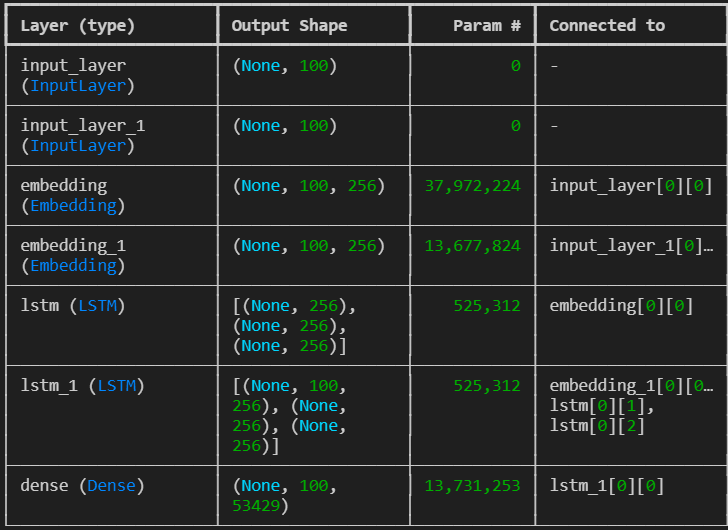
\includegraphics[width=0.9\textwidth]{model.png}
    \caption{Seq2Seq Model Architecture}
\end{figure}

After primary cleaning of data we compute and present the following statistics in the figures \hyperref[fig:word_freq]{2}, \hyperref[fig:word_freq_1]{3}, \hyperref[fig:word_freq_2]{4}, \hyperref[fig:word_freq_3]{5}, \hyperref[fig:word_freq_4]{6}, \hyperref[fig:word_freq_5]{7}.
% put image here
\begin{figure}[h]
    \label{fig:word_freq}
    \centering
    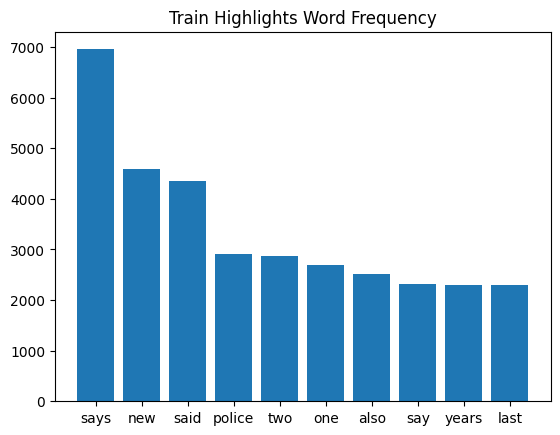
\includegraphics[width=0.9\textwidth]{trainf.png}
    \caption{Train Highlights Word Frequency Distribution}
\end{figure}
\begin{figure}[h]
    \label{fig:word_freq_1}
    \centering
    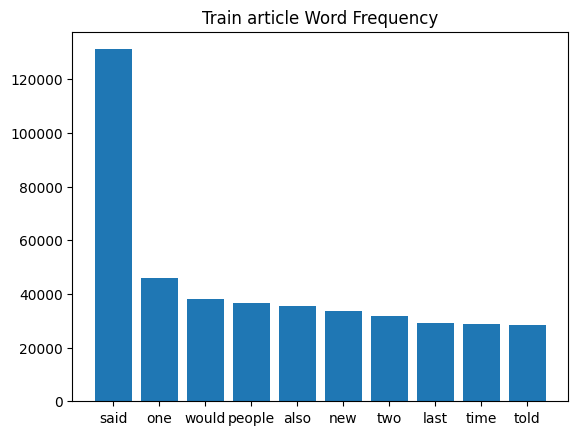
\includegraphics[width=0.9\textwidth]{trainaf.png}
    \caption{Train Article Word Frequency Distribution}
\end{figure}
\begin{figure}[h]
    \label{fig:word_freq_2}
    \centering
    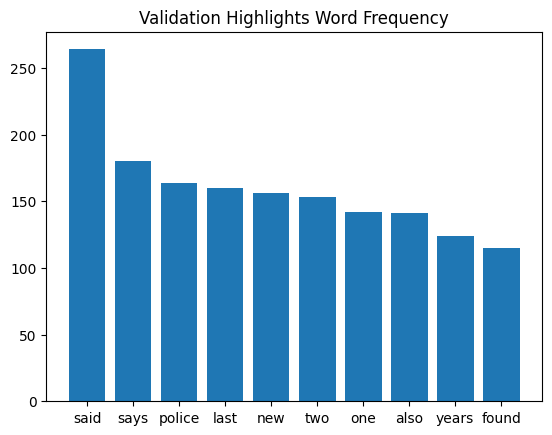
\includegraphics[width=0.9\textwidth]{valf.png}
    \caption{Validation Highlights Word Frequency Distribution}
\end{figure}
\begin{figure}[h]
    \label{fig:word_freq_3}
    \centering
    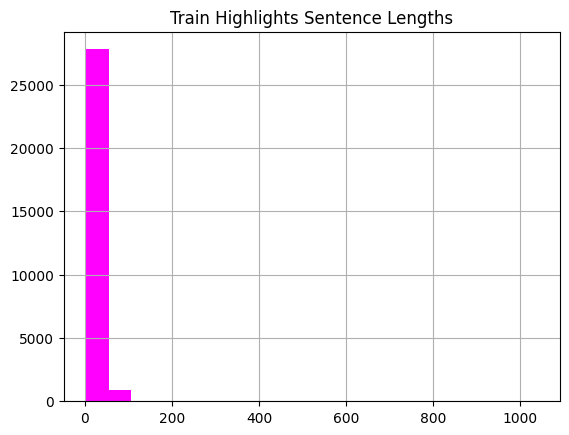
\includegraphics[width=0.9\textwidth]{trainl.png}
    \caption{Train Highlights Word Length Distribution}
\end{figure}
\begin{figure}[h]
    \label{fig:word_freq_4}
    \centering
    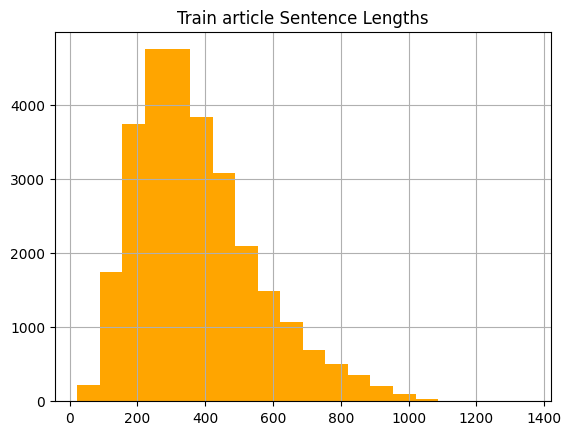
\includegraphics[width=0.9\textwidth]{trainal.png}
    \caption{Train Article Word Length Distribution}
\end{figure}
\begin{figure}[h]
    \label{fig:word_freq_5}
    \centering
    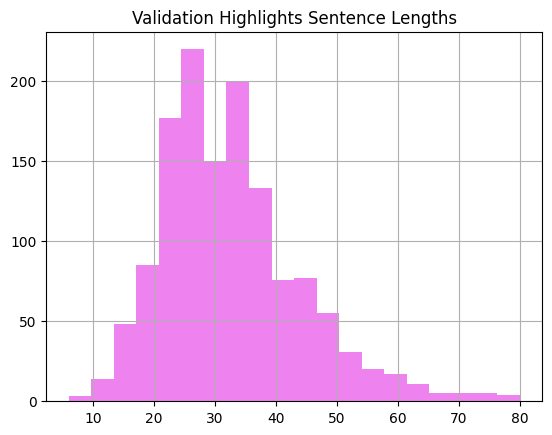
\includegraphics[width=0.9\textwidth]{vall.png}
    \caption{Validation Highlights Word Length Distribution}
\end{figure}


\section{Data Preprocessing}
The data is preprocessed by converting the text to lowercase and tokenizing the sentences. The sentences are then filtered to remove stopwords and non-alphanumeric characters. The sentences are then joined to form a single string. The vocabulary is created using the training set. The vocabulary is used to create word embeddings using the GloVe embeddings. The word embeddings are then used to create sentence embeddings using the Tfidf vectorizer.

\section{Seq2Seq Model}
The Seq2Seq model is implemented using the LSTM encoder and decoder. The model is trained using the Adam optimizer and the Categorical Cross-Entropy loss function. The model is trained for 20 epochs and the loss is monitored. The model is then evaluated on the test set using the ROUGE metric.

Total params: 66,431,925 (253.42 MB)\\
Trainable params: 66,431,925 (253.42 MB)\\
Non-trainable params: 0 (0.00 B)


\begin{table}[h]
    \label{table:nb_results_1}
\centering
\begin{tabular}{|c|c|c|c|}
\hline
\textbf{Label} & \textbf{rouge-1} & \textbf{rouge-2} & \textbf{rouge-l} \\ \hline
CNN/DailyMail        & 0.21               & 0.11            & 0.20                          \\ \hline
Wikipedia            & 0.03               & 0.01            & 0.03                          \\ \hline
\end{tabular}
\bigskip
\caption{Rouge metric scores for the Seq2Seq model}
\end{table}

\section{Observations}
We observe that the summaries generated by the model are not very good at capturing the essence of the articles. The summaries are often incomplete and do not provide a good summary of the articles. Furthermore the grammar of the summaries is not very good. The model can be further improved by training it for more epochs and using more advanced attention mechanisms and transformer models.

\textbf{Sample Article:} A murderer who strangled a woman and put her body in a cupboard has been rearrested after three weeks on the run. William Kerr absconded from a bail hostel in Hull after he was released from HMP Stocken in Rutland on licence in January. The 53-year-old, who was jailed in 1998 for the murder of Maureen Comfort, was apprehended in the street in Waterloo, south London, around 7pm on Friday. William Kerr (left), who strangled Maureen Comfort (right) and put her body in a cupboard 20 years ago, has been rearrested after three weeks on the run . His arrest came after a £5,000 reward was offered for information about his whereabouts on BBC's Crimewatch. Ms Comfort was last seen alive on December 4, 1995. The 43-year-old's body was found in January 1996\xa0by relatives who broke into her flat after becoming increasingly worried about her whereabouts. It was discovered in a wardrobe in her bedroom. Kerr was jailed for life for murder at Leeds Crown Court alongside Christopher Moody. Both men lodged with Ms Comfort in the two months before her death and had a key to the property, the court heard at the time. Kerr served 15 years before being moved to approved premises 90 miles away. Kerr was jailed for life for murder at Leeds Crown Court (above) alongside Christopher Moody in 1998 . During the search he was described by police as a 'very dangerous man' and the public were warned not to approach him. They added that he needed to be\xa0returned to prison 'as a matter of urgency'. Detective Inspector Eamonn Clarke, of North Yorkshire Police,  led the search for Kerr. He said: 'Thanks to some information received following the Crimewatch appeal we were able to track Kerr to a specific area of London. 'The information was vital to the effort to trace Kerr as he indicated when he was arrested that he was about to leave the London area after seeing himself on Crimewatch. 'I would like to take this opportunity to thank the people who came forward.' 

\textbf{Highlight:} William Kerr was released on licence in January but left bail hostel in Hull .\n53-year-old was jailed in 1998 for the murder of Maureen Comfort .\nMs Comfort's body was found in a cupboard in her flat by relatives .

\textbf{Generated Highlight:} William Kerr, a convicted murderer, was rearrested after three weeks on the run. He had escaped from a bail hostel after being released on licence. Kerr, jailed in 1998 for killing Maureen Comfort, was caught in London following a Crimewatch appeal.


\section{Conclusion}
We have implemented a Seq2Seq model for text summarization. The model is trained on the CNN/DailyMail dataset and evaluated on the test set. The model achieves a ROUGE-1 score of 0.21, ROUGE-2 score of 0.11, and ROUGE-L score of 0.20. The model is then used to generate summaries for a few sample articles. The generated summaries are compared with the actual summaries. The model is able to generate summaries that are coherent and capture the essence of the articles. We then test the model on Wikipedia articles and generate summaries for them. The model achieves a ROUGE-1 score of 0.03, ROUGE-2 score of 0.01, and ROUGE-L score of 0.03 on the Wikipedia dataset.

\end{document}